\chapter{Analyse de séries de données de débits}

\section{Explication}
\begin{itemize}
    \item \underline{\textbf{Temps de retour moyens :}} 2 à 5 ans
    \item \underline{\textbf{Temps de retour rares :}} 10, 30, 100, 300 ans, \dots ! Cela dépend surtout des objectifs de protection.
\end{itemize}

\section{Séparation des crues}
\begin{figure}[H]
    \centering
    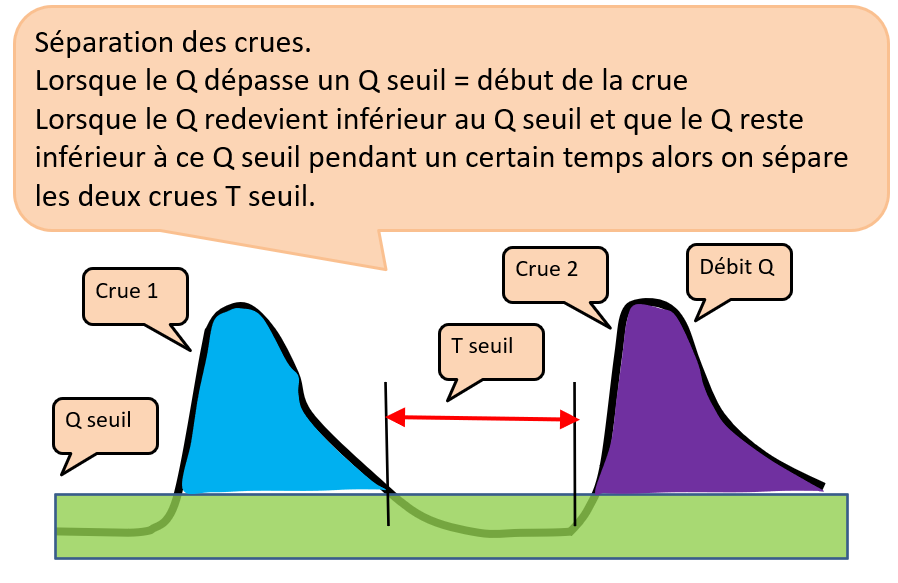
\includegraphics[width=17cm]{separationCrue.png}
    \label{fig:separationCrues}
\end{figure}

\newpage

\section{Questions intuitives sur les temps de retour}
Si on prend l'exemple suivant :
\begin{figure}[h!]
    \centering
    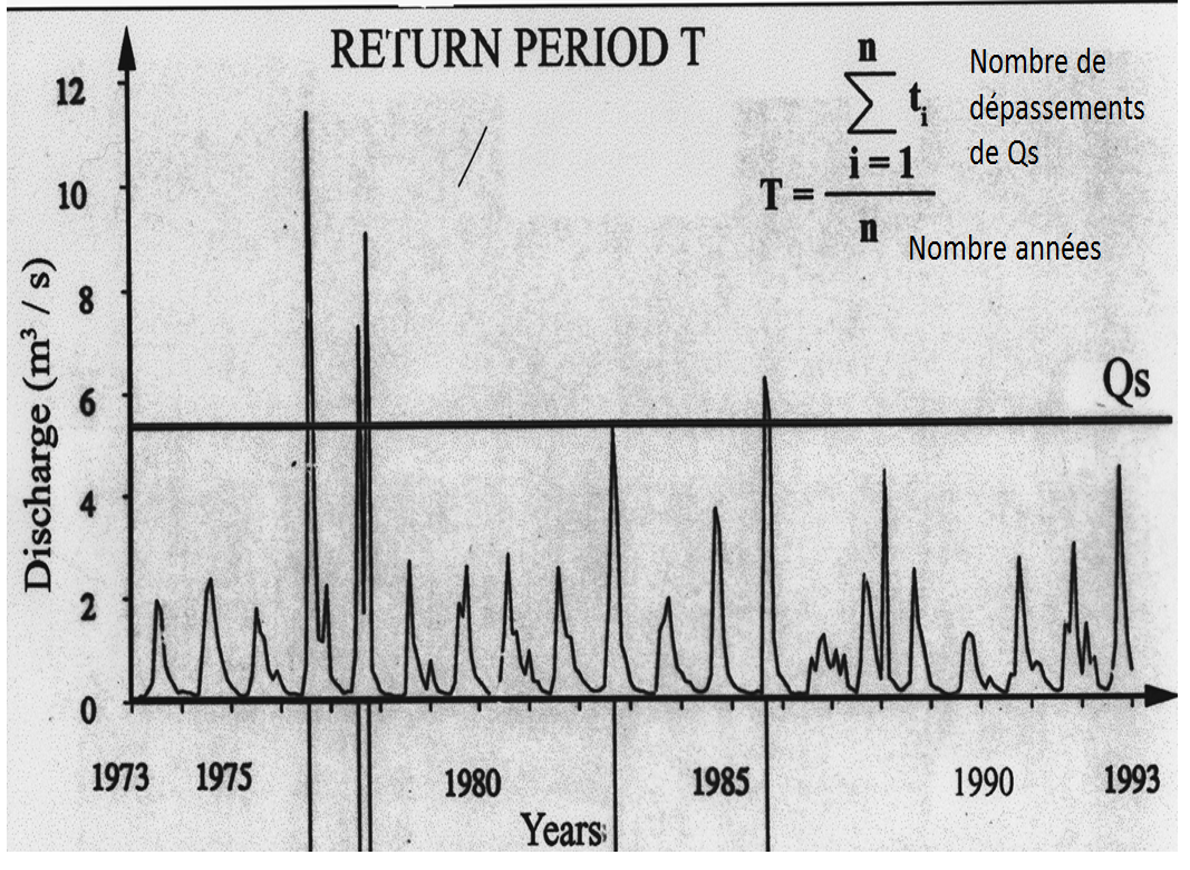
\includegraphics[width=10cm]{returnPeriodT.png}
    \caption{Graphique des débits maximums par jour}
    \label{fig:graphiqueExemple}
\end{figure}

\begin{itemize}
    \item Si on prend une période de 20 ans ; le seuil $Q_s$ est dépassé 4 fois. Donc $T_{Q_{s}} = 20/4 = 5$ ans
    \item Temps du plus gros débit : $T_{Q_{s}} = 20/1 = 20$
    \item Temps du 2\ieme gros débit : $T_{Q_{s}} = 20/2 = 10$
    \item Probabilité moyenne de dépasser le plus gros débit : $P = 1/20$
    \item Probabilité moyenne de plus dépasser le plus gros débit : $F=1-(1/20)$
\end{itemize}

\paragraph{Formule de Hazen :} Questions possibles :
\begin{itemize}
    \item Avez-vous une chance de 20 ans d'observer une crue avec un T>20 ans ? \\
    \underline{Réponse :} oui 
    \item Avec la formule de Hazen, quel est le temps de retour $T$ du plus gros débit observé pendant ces 20 ans ? \\
    \underline{Réponse :} $T = \cfrac{20}{1-0.5} = 40$ ans
\end{itemize}

\section{Séries annuelles, avec débits maximaux}

\subsection{Procédure pour déterminer et extrapoler les temps de retour}
\begin{enumerate}
    \item \textbf{\underline{Vérification de la stationnarité des données statistiques :}} \\
    \begin{itemize}
        \item Tracer le graphique des débits maximum par années comme la Fig XX
        \item Vérification que cela ne varie par en fonction des années (courbe de tendance)
        \item Visualiser l'évolution des crues de pointe en fonction des années donne un bon aperçu d'une dérive quelconque
        \item \Warning Si les données ne sont pas stationnaires ; cela ne sert à rien de continuer la procédure pour déterminer les débits extrapolés
    \end{itemize}
    \bigskip
    \item \textbf{\underline{Vérification de l'homogénéité des données statistiques :}}
    \begin{itemize}
        \item Tracer le graphique des débits maximum par années comme la Fig XX
        \item Vérification optionnelle (car implique d'avoir les débits maximaux mensuels)
        \item Vérification que cela ne varie par en fonction des années (courbe de tendance)
        \item Visualiser l'évolution des crues de pointe en fonction des années donne un bon aperçu d'une dérive quelconque
    \end{itemize}
\end{enumerate}

\section{Séries gonflées}
Une série gonflée est une série de données statistiques où nous avons \underline{2 ou plus débits maximaux par année}.

\section{Séries tronquées}
Une série tronquée est une série de données statistiques où les \underline{débits sont supérieurs à $Q_\text{seuil}$.} \\
\Warning Si le seuil est trop bas, on prend des débits très fréquents et des débits extrêmes ; qui ne sont peut-être pas homogène. \\
On prend les séries tronquées pour obtenir les débits fréquents de temps de retour faible; voire inférieur au temps de retour années. \\
Privilégiez les séries tronquées aux séries gonflées.